%% Introduction to latex facilities.
%% Sat 31 Dec 2005
%% Stephen Eglen.

%% Text following a percent sign (%) until the end of line is treated
%% as a comment.

\documentclass{article}

%%%%%%%%%%%%%%%%%%%%%%%%%%%%%%%%%%%%%%%%%%%%%%%%%%%%%%%%%%%%%%%%%%%%%%
%% This section is called the preamble, where we can specify which
%% latex packages we required.  Most (but not of all) of the packages
%% below should be fairly standard in most latex documents.  The
%% exception is xspace and the new \latex command, which you probably
%% do not need.
%%%%%%%%%%%%%%%%%%%%%%%%%%%%%%%%%%%%%%%%%%%%%%%%%%%%%%%%%%%%%%%%%%%%%%

%% Better math support:
\usepackage{amsmath}

%% Bibliography style:
\usepackage{mathptmx}           % Use the Times font.
\usepackage{graphicx}           % Needed for including graphics.
\usepackage{url}                % Facility for activating URLs.

%% Set the paper size to be A4, with a 2cm margin 
%% all around the page.
\usepackage[a4paper,margin=2cm]{geometry}

%% Natbib is a popular style for formatting references.
\usepackage{natbib}
%% bibpunct sets the punctuation used for formatting citations.
\bibpunct{(}{)}{;}{a}{,}{,}

%% textcomp provides extra control sequences for accessing text symbols:
\usepackage{textcomp}
\newcommand*{\micro}{\textmu}
%% Here, we define the \micro command to print a text "mu".
%% "\newcommand" returns an error if "\micro" is already defined.

%% This is an example of a new macro that I've created to save me
%% having to type \LaTeX each time.  The xspace command provides space
%% after the word LaTeX where appropriate.
\usepackage{xspace}
\providecommand*{\latex}{\LaTeX\xspace}
%% "\providecommand" does nothing if "\latex" is already defined.


\usepackage[utf8]{inputenc}

\newcommand{\ie}{i.e.,\ }
\newcommand{\eg}{e.g.,\ }
\newcommand{\ps}{P/S\ }
\newcommand{\cf}{c.f.\ }
\newcommand{\fs}{4Sensing}

\usepackage{verbatim}
\usepackage{fancyvrb}
\DefineVerbatimEnvironment%
      {VrbSnippet}%
      {Verbatim}%
      {fontsize=\scriptsize}

\newcommand{\tm}[1]{\texttt{#1}}

      
%%%%%%%%%%%%%%%%%%%%%%%%%%%%%%%%%%%%%%%%%%%%%%%%%%%%%%%%%%%%%%%%%%%%%%
%% Start of the document.
%%%%%%%%%%%%%%%%%%%%%%%%%%%%%%%%%%%%%%%%%%%%%%%%%%%%%%%%%%%%%%%%%%%%%%

\begin{document}
\title{4Sensing - Documentação}
\maketitle

\section{Operação do Simulador}

O simulador pode ser operado a partir do Eclipse ou Ant. Um bug no plugin Greclipse com tipos enumerados (\url{http://netbeans.org/bugzilla/show_bug.cgi?id=189275}) não permite compilar (inicialmente) o código no IDE.  Eventualmente o erro desaparece.  A versão mais recente do plugin Greclipse possivelmente já não tem este problema, mas só é suportado no Eclipse 3.6 que tem bloqueios frequentes em OS X.

As próximas secções  documentam as tarefas Ant e scripts para operação do simulador.

\subsection{Tarefas Ant}

\subsubsection{deploy}
Compila o código e copia binários e configurações para pasta \tm{bin}.

\subsubsection{clean}
Lista as classes compiladas (pastas \tm{antbin} e \tm{bin})

\subsubsection{run}\label{sec:taskrun}
Executa o script run.sh para lançar simulações - ver \ref{sec:runsh}. A tarefa é configurada por três parâmetros definidos no início em \tm{build.xml}.

\begin{enumerate}
\item \tm{runid}: string que define o nome da experiência. É utilizada para definir o path para o ficheiro de output  - ver secção \ref{sec:output}
\item \tm{runenv}: string que define o ambiente de execução. É utilizado para definir o ficheiro \tm{runenv\_[runenv].sh} a executar para definição dos parâmetros da JVM
\item \tm{runtimes}: número de simulações a correr para cada setup
\end{enumerate}

\subsubsection{pack/packsrc}
Tarefas utilizadas para gerar arquivos tgz - completo ou apenas source, respectivamente - para instalação num ambiente remoto. 
Antes do packaging, é verificado se o repositório svn está sincronizado - \ie se o output de \tm{svn status} é vazio. A verificação é utilizada em conjunto com um svn hook para garantir que os resultados de simulações são marcadas com a versão do código no repositório (o hook limita-se a criar o ficheiro /src/4sensing-ver.properties com a versão actual no repositório).

NOTA: o svn hook (ficheiro \tm{util/post-commit}) actualmente não está instalado no svn da faculdade.

\subsection{Execução da Simulação - run.sh}\label{sec:runsh}

A simulação é lançada executando \tm{java [classe de simulação]}, colocando no classpath todos os jars definidos na pasta \tm{lib} e classes na pasta \tm{bin}. É conveniente configurar a JVM com pelo menos 800Mb de heap.
%TODO: Definir classe de simulação

O script \tm{run.sh} foi criado para facilitar a execução de uma simulação, ou várias simulações em sequência. Recebe 3 argumentos que correspondem aos três parâmetros definidos em \ref{sec:taskrun}:  \tm{runid}, \tm{runenv}, \tm{runtimes}. O script define um ou mais setups - variável \tm{SETUPS}, definida no início. No ciclo de execução (ciclo \tm{while} na linha 43), define-se os simuladores a correr - por exemplo pode correr-se diferentes estratégias de distribuição em sequência (ver código comentado).

Os logs gerados por cada simulação (relevantes para debugging) são colocados na pasta \tm{logs} com o seguinte nome:

\begin{Verbatim}
[run name]_[data/hora]_[nome simulador]_[FQN da classe de setup]_ \
[número de sequência da simulação].log
\end{Verbatim}

O nome do simulador é definido em \tm{run.sh} (na chamada à função \tm{run}) - normalmente é uma string que descreve sumariamente o simulador \eg \tm{SUMO\_Centralized} para o simulador SUMO utilizando o modelo centralizado.

Os resultados da simulação são colocados dentro na pasta \tm{results} numa estrutura em árvore com a configuração seguinte:

\begin{Verbatim}
[FQN da classe de setup]/run_[run name]_[data/hora]/[FQN da classe de simulação]
\end{Verbatim}

O conteúdo dos resultados é definido na classe de setup.

\begin{comment}
%TODO
\subsection{Scripts Auxiliares}

\begin{itemize}
\item \tm{log.sh}
\item \tm{etc.sh}
\end{itemize}
\end{comment}

\subsection{Integração com SUMO/TAPAS Cologne}\label{sec:sumo-tapas}
Para utilizar os dados do TAPAS Cologne é necessário correr previamente a simulação SUMO para este cenário. A simulação é corrida uma única vez para uma dada parametrização, e o output é posteriormente utilizado para as simulações 4Sensing. Para correr uma simulação SUMO:

\begin{enumerate}
\item Expandir o arquivo com o cenário TAPAS Cologne 0.0.3
\item Copiar conteúdo da pasta \tm{sumo}, no projecto 4Sensing, para a pasta TAPASCologne-0.0.3
\item Editar \tm{TAPASCologne-0.0.3/4Sensing.cfg}, tag \tm{<end value="x"/>}, para definir a duração da simulação. Os dados disponibilizados livremente cobrem 2 horas de simulação - de 21600s a 28800s
\item Editar \tm{TAPASCologne-0.0.3/input\_additional.add.xml} para configurar os dois tipos de output utilizados pelo 4Sensing:
\begin{enumerate}
\item Na tag \tm{meandata-edge} \footnote{Documentação em \url{http://sourceforge.net/apps/mediawiki/sumo/index.php?title=SUMO_OUTPUT_EDGELANE_TRAFFIC}} é definido a periodicidade para as estatísticas de segmentos (actualmente 5 minutos) e o nome do ficheiro de output
\item Na tag \tm{vtyperobe}\footnote{Documentação em \url{http://sourceforge.net/apps/mediawiki/sumo/index.php?title=SUMO_OUTPUT_VTYPEPROBE}} é definida a periodicidade da amostragem de posição/velocidades para os veículos (actualmente 5 segundos) e o nome do ficheiro de output
\end{enumerate}
\item Correr simulador: \tm{sumo -c 4Sensing.cfg}
\item Copiar resultados da simulação para a raiz do projecto 4Sensing
\item Copiar modelo da rede viária para pasta \tm{sumo} no projecto 4Sensing: 

\tm{TAPASCologne-0.0.3/road/no\_internal/koeln\_bbox.net.xml}
\end{enumerate}

\section{Output e Gráficos}\label{sec:output}

O output da simulação é definido na classe de setup - o método \tm{setupCharts} devolve uma lista de especializações da classe \tm{sensing.persistence.simsim.Metric} que são responsáveis por compilar métricas, a sua visualização em ambiente gráfico e a persistência em ficheiro.

No caso das simulações SUMO, o output é simplesmente a compilação dos resultados da query em ficheiro, resultando num ficheiro por simulação. O ficheiro contém uma linha por cada resultado, com valores separados por \tm{tab}. Os valores registados para cada resultado são definidos no método \tm{outputResult}, na chamada ao método \tm{lineOut.newLine}. Por exemplo, em \tm{SUMOTrafficSpeedSetup}:

\begin{Verbatim}
lineOut.newLine([s.count,
	s.vCount,
	s.minSpeed * 3.6, ...])
\end{Verbatim}

Isto resulta num ficheiro \tm{results\_[sim].gpd} na pasta definida em \ref{sec:runsh}, em que \tm{sim} é o número de sequência da simulação. Para o setup \tm{SUMOTrafficSpeedSetup} cada linha do ficheiro contém a seguinte informação:

\begin{enumerate}
\item Número de amostras agregadas no resultado
\item Número de veículos que contribuem amostras para o resultado
\item Velocidade mínima em Km/h, calculada pela tabela virtual
\item Velocidade máxima em Km/h, calculada pela tabela virtual
\item Velocidade média em Km/h, calculada pela tabela virtual
\item Desvio padrão da velocidade em Km/h, calculada pela tabela virtual
\item Velocidade mínima em Km/h, utilizando os traces SUMO (não é utilizado)
\item Velocidade máxima em Km/h, utilizando os traces SUMO (não é utilizado)
\item Velocidade média em Km/h, utilizando os traces SUMO (não é utilizado)
\item Desvio padrão da velocidade em Km/h, utilizando os traces SUMO (não é utilizado)
\item Número de amostras disponíveis nos traces SUMO (não é utilizado)
\item Velocidade média - obtida através das estatísticas SUMO
\item Taxa de ocupação média, obtida através das estatísticas SUMO
\item Densidade média, obtida através das estatísticas SUMO
\item Número de amostras, obtida através das estatísticas SUMO
\item Velocidade máxima para o segmento, informação estática obtida no modelo de estradas do SUMO
\item Número de faixas do segmento,  informação estática obtida no modelo de estradas do SUMO
\item Comprimento do segmento, informação estática obtida no modelo de estradas do SUMO
\item Presença de semáforos? 1 - Sim, 0 - Não, informação estática inferida do modelo de estradas do SUMO
\item Segmento totalmente contido na área da query? 1 - Sim, 0 - Não, informação estática inferida do modelo de estradas do SUMO
\item Identificador do segmento
\item Timestamp do resultado
\end{enumerate}



\subsection{Pós-Processamento}\label{sec:posproc}
O formato de output descrito acima pode ser utilizado directamente para gerar gráficos usando gnuplot \eg gráficos de dispersão. Para gráficos mais elaborados é necessário pré-processar os dados, pelo que foi implementado um conjunto de scripts Groovy para esse efeito. Os scripts específicos para a versão actual do SpeedSense \ie extracção da velocidade média por segmento, estão no package \tm{sensing.persistence.util.sumo.segmentspeed2}. 

O processo normal para a criação de gráficos após a execução de simulações será o seguinte:

\begin{enumerate}
\item Processamento do output para acrescentar dados de referência relativa a 100\% de participação  - ver \ref{sec:refdata}
\item Processamento do output do passo anterior para gerar ficheiros fonte para gnuplot - ver \ref{sec:graph} e \ref{sec:coverage}
\item Gerar e executar scripts gnuplot - exemplos em \tm{graphs/segmentspeed2} na pasta do projecto
\end{enumerate}

É necessário anteceder o passo 1 com a execução do script \tm{SegmentRatingOut} para cálculo do \emph{comprimento dinâmico} dos segmentos. Este passo é necessário apenas uma vez após a simulação SUMO.

\subsubsection{sensing.persistence.util.sumo.SegmentRatingOut}\label{sec:segmentratingout}
Executado pela tarefa Ant \tm{segrate}. Determina o comprimento dinâmico dos segmentos para uma área de pesquisa e tempo de simulação, utilizando como fonte os traces SUMO (output \tm{vtypeprobe} definido em \ref{sec:sumo-tapas}). No exemplo abaixo, é gerado o comprimento dinâmico para os primeiros 30 minutos de simulação.

\begin{Verbatim}
String mapData = "koeln_bbox_net.xml"
String vProbeData = "sumocfg3_vtypeprobe_5s_nointernal.xml"
int endTime = 23400
...
Rectangle2D qArea = new Rectangle2D.Double(minLon, minLat, width, height);
String outFile = "segmentRating_1800.tsv"
\end{Verbatim}

\subsubsection{sensing.persistence.util.sumo.segmentspeed2.RefData}\label{sec:refdata}
Executado pela tarefa Ant \tm{ss\_refdata}. O script acrescenta a cada resultado da query os dados relativos a 100\% de participação. Em particular:

\begin{enumerate}
\item Erro da velocidade média (a diferença entre a velocidade média do resultado e o mesmo valor para 100\% de participação)
\item O comprimento dinâmico do segmento
\item Número de amostras agregadas no resultado - valor obtido com 100\% de participação
\item Número de veículos que contribuem amostras para o resultado - valor obtido com 100\% de participação
\item Velocidade média - valor obtido com 100\% de participação
\item Desvio padrão da velocidade - valor obtido com 100\% de participação
\end{enumerate}

No inicio do scipt é definida a localização dos dados das simulações e a pasta para output

\begin{Verbatim}
String setupName = "segmentspeed2.SUMOTrafficSpeedSetup_10m"
String baseRunName = "run_segspeed2_10m08-06-2011-13-16-08" 
String baseSimId = "0"
String runName = "run_segspeed2_10m08-06-2011-13-16-08"
String simId = "0"
String segRating = "segmentRating_1800.tsv"
String outDir = "results/segspeed2/rateresults"
def rates = [1,2,3,5,7,10,100]
\end{Verbatim}

\begin{itemize}
\item \tm{setupName} refere a classe setup, sem o número que identifica a percentagem de participação. O valor será prefixado com:
\tm{sensing.persistence.simsim.speedsense.sumo.setup.}
\item \tm{baseRunName} é o nome do run onde se encontram os dados de referência - 100\% de participação. Normalmente será igual a \tm{runName}
\item{baseSimId} é o número de sequência da simulação para os dados de referência
\item \tm{runName} é o nome do run onde se encontram os dados a processar
\item{baseSimId} é o número de sequência da simulação a processar
\item \tm{outDir} é a pasta de saída
\item \tm{rates} define as percentagens de participação a considerar - usado em conjunto com o prefixo \tm{setupName}
\end{itemize}

É criado na pasta \tm{outDir} um ficheiro para cada percentagem de participação (rate) com o nome 

\tm{[setupName]\_err\_[rate].gpd}.

\subsubsection{sensing.persistence.util.sumo.segmentspeed2.Graph}\label{sec:graph}
Executado pela tarefa Ant \tm{ss\_graph}. O objectivo do script é gerar dados processados, num formato apropriado para gnuplot, para criar vários tipos de gráficos a partir da classificação dos resultados - \eg ver figuras \ref{fig:speedrate_errorkmh}, \ref{fig:sumoerror} e \ref{fig:hist_speedrate_100}. O input do script será  o conjunto de ficheiros gerados pelo script \tm{RefData}.

No script é usada uma função de classificação que separa os resultados em diferentes classes (bins) e para cada classe é calculado um valor, através de uma função de sumarização, que representa os dados englobados. Por exemplo para calcular o erro médio em Km/h, relativo a 100\% de participação, para diferentes classes de racio de velocidades (velocidade média/velocidade máxima) - figura \ref{fig:speedrate_errorkmh} - é usada a função de classificação \tm{binfSpeedRate} e a função de sumarização \tm{errorKmh}. Para o gráfico da figura \ref{fig:sumoerror}, é usada a função de sumarização \tm{sumoErrorKmh}.

\begin{figure}[h!]
	\centering
	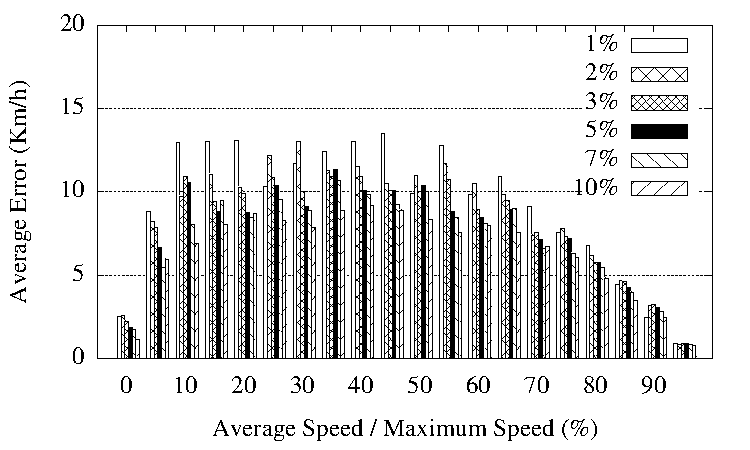
\includegraphics[width=0.75\textwidth]{figs/ss_speedrate_errorkmh.pdf}
	\caption{Relação entre o racio de velocidades e o erro médio durante uma simulação}
	\label{fig:speedrate_errorkmh}
\end{figure}

A parametrização é definida no início do script:

\begin{Verbatim}
String inDir = "results/segmentspeed2/rateresults"
String setupName = "segmentspeed2.SUMOTrafficSpeedSetup"
String metricName = "hist_speedrate_errorkmh_all"
String outDir = "results/segmentspeed2/ss_error_2"
rates = [1,2,3,5,7,10,50,100]
\end{Verbatim}

\begin{itemize}
\item \tm{inDir} identifica a pasta onde estão os resultados - corresponde a \tm{outdir} do script \tm{RefData}
\item \tm{outDir} define pasta onde serão guardados os resultados do script
\item \tm{setupName} o nome da classe setup, será igual ao valor \tm{setupName} definido em \tm{RefData}
\item \tm{metricName} é o nome da métrica - utilizado para gerar os nomes dos ficheiros de output
\item \tm{rates} define as percentagens de participação a considerar - usado em conjunto com o prefixo \tm{setupName} para obter os ficheiros fonte
\end{itemize}

O script pré-define um conjunto de funções de classificação/sumarização que poderá ser aumentado com novas funções. Para configurar o script com as funções pretendidas, altera-se a chamada à função \tm{run} (linha 169), substituindo os identificadores \tm{binfSpeedRate} e \tm{errorKmh} pelas funções pretendidas.

\begin{Verbatim}
def meanerror = rates.collect{[it, run(it, {vals-> true}, binfSpeedRate, errorKmh, outfStats )] }
\end{Verbatim}

Pode também ser definida uma função de filtragem - passada como segundo argumento da função \tm{run}. Por exemplo para utilizar apenas dados relativos a segmentos com sinais, utiliza-se a função: \tm{\{vals -> vals.edgetl.equals("1")\}}. Esta é a base para criar o gráfico da figura \ref{fig:hist_speedrate_100}.

Os dados para cada percentagem de participação (rate) são processados e os resultados guardados na pasta de output em ficheiros individuais com o nome \tm{ss\_[metricName]\_[rate].gpd}. Estes ficheiros - que são a base do gráfico das figura \ref{fig:speedrate_errorkmh} e \ref{fig:hist_speedrate_100} - contém uma linha por cada classe com os seguintes valores: o valor da classe (\eg 10 representa os racios de velocidade no intervalo [10,20[), o valor de sumarização, a frequência da classe e os valores mínimos e máximos para a funcão de sumarização. 

Para além dos ficheiros por percentagem de participação, é gerado um ficheiro com os dados "globais" (\tm{ss\_[metricName].gpd}) \ie independente de classificação - a função de sumarização é aplicada à totalidade dos resultados para cada rate. Para o exemplo da figura \ref{fig:sumoerror}, o ficheiro irá conter, para cada percentagem de participação, o erro médio global em Km/h.

Na pasta \tm{graphs/segmentspeed2} do projecto encontram-se scripts gnuplot para gerar os gráficos usados como exemplo:

\begin{itemize}
\item \tm{ss\_speedrate\_errorkmh.gp} para o gráfico na figura \ref{fig:speedrate_errorkmh}
\item \tm{ss\_hist\_sumoerror.gp} para o gráfico na figura \ref{fig:sumoerror}
\item \tm{ss\_hist\_speedrate\_100.gp} para o gráfico na figura \ref {fig:hist_speedrate_100}
\end{itemize}

\begin{figure}[t!]
	\centering
	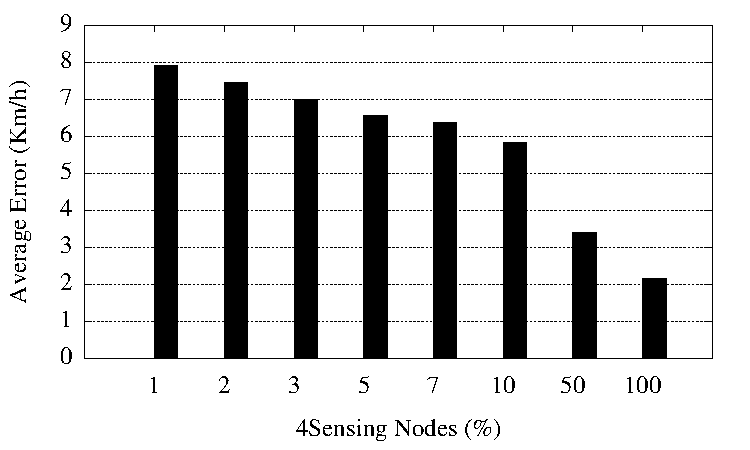
\includegraphics[width=0.66\textwidth]{figs/ss_hist_sumoerror.pdf}
	\caption{Erro médio relativo às estatísticas do SUMO}
	%Average error relative to SUMO statistics
	\label{fig:sumoerror}
\end{figure}

\begin{figure}[h!]
	\vspace{-2mm}
	\centering
	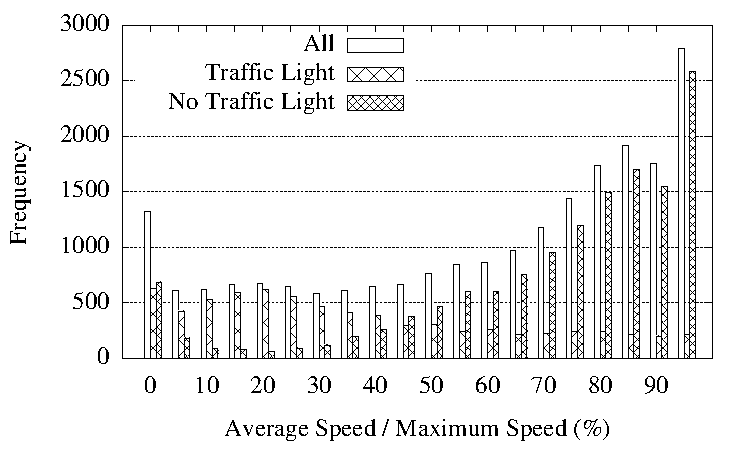
\includegraphics[width=0.75\textwidth]{figs/tt_hist_speedrate_100.pdf}
	\caption{Ocorrência dos diferentes racios de velocidade durante uma simulação - 100\% veículos \fs{}}
	%Occurrence of different speed rates during one simulation - 100\% \fs{} vehicle rate
	\label{fig:hist_speedrate_100}
\end{figure}


\subsubsection{sensing.persistence.util.sumo.segmentspeed2.CoverageVsErrorGraph}\label{sec:coverage}
Executado pela tarefa Ant \tm{ss\_coverage}. O objectivo do script é gerar os dados necessários para a criação de gráficos de cobertura com gnuplot.
A configuração é definida no início do script:

\begin{Verbatim}
String inDir = "results/segspeed2/rateresults"
String setupName = "segmentspeed2.SUMOTrafficSpeedSetup_10m"
String metricName = "dinamic_length_coverage"
String outDir = "results/segspeed2/ss_error_2"
String segRating = "segmentRating_1800.tsv" 
def rates = [1,2,3,5,7,10]
\end{Verbatim}

\begin{itemize}
\item \tm{inDir} identifica a pasta onde estão os resultados - corresponde a \tm{outdir} do script \tm{RefData}
\item \tm{setupName} o nome da classe setup, será igual ao valor \tm{setupName} definido em \tm{RefData}
\item \tm{metricName} é o nome da métrica - utilizado para gerar os nomes dos ficheiros de output
\item \tm{outDir} define a pasta onde serão guardados os resultados
\item \tm{segRating} é o nome do ficheiro com os comprimentos dinâmicos por segmento, gerados pelo script \tm{SegmentRatingOut} - ver \ref{sec:segmentratingout}
\item \tm{rates} define as percentagens de participação a considerar
\end{itemize}

Os dados para cada percentagem de participação (rate) são processados e os resultados guardados na pasta de output em ficheiros individuais com o nome \tm{ss\_[metricName]\_[rate].gpd}. Em cada ficheiro, a primeira coluna representa a classe de erro em Km/h. As restantes 10 colunas contém a taxa de cobertura para o nível de erro correspondente, em que cada coluna representa um racio de velocidades (de 10 a 100, com intervalo de 10). Estes ficheiros são a base para gerar o gráficos  da figura \ref{fig:error_coverage_all}. Para um exemplo de script gnuplot para criação deste gráfico, ver o ficheiro \tm{ss\_coverage\_all.gp} na pasta \tm{graphs/segmentspeed2} do projecto.

\begin{figure}[h!]
	\centering
	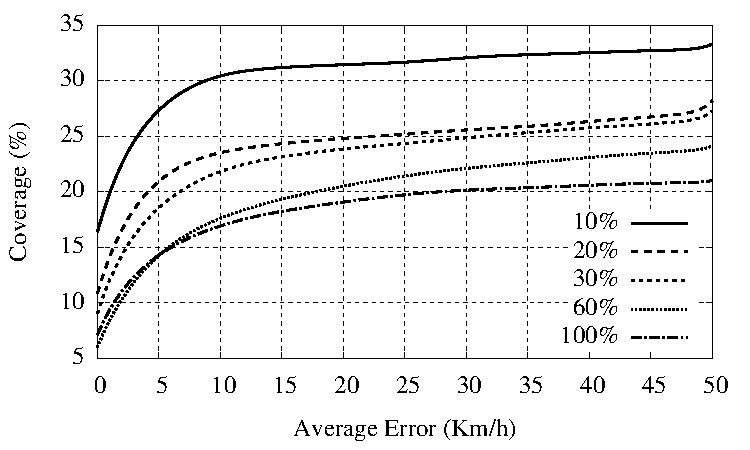
\includegraphics[width=0.75\textwidth]{figs/ss_speedrate_coverage.pdf}
	\caption{Erro médio vs racio de cobertura - considerando todos os resultados}
%	\caption{Average error vs coverage rate - considering all query results}
	\label{fig:error_coverage_all}
\end{figure}

Para cada percentagem de participação, é também gerado um ficheiro (\tm{ss\_[metricName]\_[rate]\_overall.gpd}) que contém a taxa de cobertura para cada racio de velocidades, independente do erro. Neste caso a primeira coluna representa a classe de racio de velocidades e a segunda representa a cobertura correspondente. Estes ficheiros são a base para gerar gráficos como na figura \ref{fig:coverage_all}.  Para um exemplo de script gnuplot para criação deste gráfico, ver o ficheiro \tm{ss\_speedrate\_coverage.gp} na pasta \tm{graphs/segmentspeed2} do projecto.

\begin{figure}[h!]
	\vspace{-2mm}
	\centering
	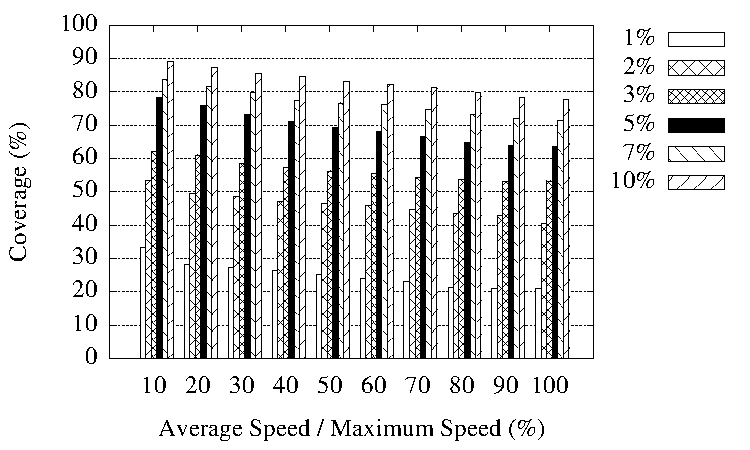
\includegraphics[width=0.75\textwidth]{figs/ss_coverage_all.pdf}
	\caption{racio de cobertura vs racio de velocidade - considerando todos os resultados}
	%Coverage rate vs speed rate - considering all query results
	\label{fig:coverage_all}
\end{figure}

\begin{comment}
\section{GUI}
%TODO: Apresentar 4sensing.properties?
\end{comment}

\section{Desenvolvimento de Cenário de Simulação}
Para ilustrar os passos necessários para criar um novo cenário de simulação é utilizado como exemplo a detecção local de congestionamentos.
O objectivo será introduzir complexidade no processamento local, de forma que os veículos forneçam informação de mais alto nível \eg os veículos podem inferir situações de congestionamento usando a frequência de paragem numa determinada janela temporal.

\begin{enumerate}
\item Criar novo tipo de nó móvel
\item Criar tabela virtual e tuplos
\item Criar setups
\end{enumerate}

\subsection{Nó Móvel}

Um novo tipo de nó móvel é definido por extensão da classe Java \tm{sensing.persistence.simsim.MobileNode}. A classe \tm{MobileNode} define a interface base para um nó móvel, em particular para a comunicação de leituras para a infraestrutura 4Sensing (método \tm{sensorInput}).

Para cenários SUMO, um nó móvel estende a classe  \tm{sensing.persistence.simsim.sumo.SUMOMobileNode}, que define adicionalmente a interface para actualização da posição/velocidade a partir da reprodução de traces SUMO.

Para gerar informação de alto nível a partir de informação dos traces será necessário estender o método \tm{update}, por exemplo colocando as leituras numa janela temporal e determinando periodicamente a frequência de paragens. A comunicação de uma leitura é feita da seguinte forma.

\begin{Verbatim}
GroovyObject m = simJ.newTuple("speedsense.CongestionDetection"); 
m.setProperty("segmentId", sampledEdge.id); 
...
sensorInput(m);
\end{Verbatim}

O metodo \tm{sensorInput} é responsável por acrescentar o timestamp e identificador do nó móvel.

\subsection{Tabela Virtual e Tuplos}
A tabela virtual e os tuplos podem ser criada em qualquer package. Para a aplicação SpeedSense estas entidades estão agrupadas no package \tm{speedsense}. Segue um exemplo para produzir tuplos \tm{CongestionDetection} que simplesmente soma o número de detecções locais produzidas por veículos.
O operador \tm{set} na fase data-source garante que apenas uma detecção por veículo (\tm{mNodeId}) será contabilizada. Na fase de agregação global, o operador \tm{set} mantém a informação dos diferentes peers recebida nos últimos 5 minutos, relativa a um segmento, e desencadeia a recomputação da agregada quando é recebida nova informação de peers descendentes.

\begin{Verbatim}
def wSize = SpeedSenseSim.setup.VT_WINDOW_SIZE
sensorInput(CongestionDetection)
dataSource{
	timeWindow(mode:periodic, size:wSize, slide:wSize)
	set(['mNodeId','segmentId'], mode:eos, ttl:1)
	groupBy(['segmentId]) {
		aggregate(CongestionDetection) { CongestionDetection d ->
			count(d, 'count')
}}}
globalAggregation{
	groupBy(['segmentId]) {
		set(['peerId'], mode:change, ttl:300)
		aggregate(CongestionDetection) { CongestionDetection d ->
			sum(d, 'count', 'count')
}}}
\end{Verbatim}

O tuplo \tm{CongestionDetecions} define os campos \tm{segmentId} e \tm{count}:
\begin{Verbatim}
package speedsense;
import sensing.persistence.core.pipeline.Tuple;

public class AggregateSpeed extends Tuple {
	String segmentId
	int count
}
\end{Verbatim}

\subsection{Setups}
O setup define o cenário de simulação:
\begin{itemize}
\item Configura a simulação
\item Define a pesquisa a executar (ou mais de uma pesquisa)
\item Define a colecção de dados de output
\end{itemize} 


\subsubsection{Configuração}
A classe base para qualquer setup é a classe \tm{sensing.persistence.simsim.SimSetup}. Para cenários SpeedSense, o setup irá extender a classe \tm{sensing.persistence.simsim.speedsense.setup.SpeedSenseSetup}.

A classe \tm{sensing.persistence.simsim.speedsense.sumo.setup.segmentspeed2.SUMOTrafficSpeedSetup} pode ser usada como referência para a criação do novo setup.

A configuração é definida no construtor da classe, definindo os parâmetros da seguinte forma:

\begin{Verbatim}
config.VT_WINDOW_SIZE = 300
\end{Verbatim}

Neste caso é configurado o parâmetro \tm{VT\_WINDOW\_SIZE} utilizado na definição da tabela virtual. Podem ser definidos parâmetros arbitrários a usar nas tabelas virtuais ou nós móveis. Existe um conjunto de parâmetros pré-definidios para um cenário SUMO:


\begin{tabular}{| l | p{0.5\textwidth} | l | }
\hline
Parâmetro & Função & Default\\
\hline
\tm{RUN\_TIME} & Tempo de execução da simulação em, segundos & 0 \\ \hline
\tm{IDLE\_TIME} & Intervalo de tempo entre o início da simulação e a execução da query & 0 \\ \hline
\tm{SIM\_SEED} & Seed para números aleatórios - equivale a \tm{Sim\_RandomSeed}, da classe \tm{Globals} do SimSim & 0L \\ \hline
\tm{NET\_SEED} & Seed para números aleatórios - equivale a \tm{Net\_RandomSeed}, da classe \tm{Globals}  do SimSim & 0L \\ \hline
\tm{SIM\_TIME\_WARP} & Determina velocidade de execução do simulador relativamente a tempo real   & 1E9 \\ \hline
\tm{TOTAL\_NODES} & Número de nós na infraestrutura fixa 4Sensing & 500 \\ \hline
\tm{MIN\_NODES\_PER\_QUAD} & Parametro específico para a estratégia de distribuição QTree & 2 \\ \hline
\tm{MIN\_NODE\_DISTANCE} & Distância mínima entre nós fixos, em metros & 250 \\ \hline
\tm{SAMPLING\_PERIOD} & Período de amostragem para um nó móvel 4Sensing, em segundo. O significado deste período depende da implementação do nó móvel & - \\ \hline
\tm{SUMO\_MNODE\_RATE} & Define o racio de participação \ie o racio de veículos SUMO que correspondem a nós 4Sensing & - \\ \hline
\tm{SUMO\_MNODE\_CLASS\_NAME} & FQN da classe que implementa o nó móvel & - \\ \hline
\tm{SUMO\_VPROBE\_SAMPLING\_PERIOD} & O período de amostragem para os traces SUMO, terá que corresponder à parametrização \tm{vtypeproble} - ver secção \ref{sec:sumo-tapas} & - \\ \hline
\tm{SUMO\_EDGESTATS\_PERIOD} & O período de actualização das estatísticas SUMO, terá que corresponder à parametrização \tm{meandata-edge} - ver secção \ref{sec:sumo-tapas} & - \\ \hline
\end{tabular}

%TODO Onde está a definição do filtro geográfico?

\subsubsection{Pesquisa}
O início da pesquisa é desencadeado pelo método  \tm{startQuery}. Para criar uma query centrada na área simulação e com 1/4 da área desta:

\begin{Verbatim}
protected void startQuery() {
	String pipelineName = "speedsense.CongestionDetectionVT";
	double centerLat = sim.world.center().y;
	double centerLon = sim.world.center().x;
	double width = 0.25 * sim.world.width;
	double height = 0.25 * sim.world.height;
	Query q = createQuery(pipelineName, centerLat, centerLon, width, height);
	runQuery(q) { CongestionDetection d -> outputResult(d)}
}
\end{Verbatim}

\subsubsection{Output}

No caso mais simples, o resultado da simulação será o registo em ficheiro dos resultados da query. Para isso instancia-se a classe \tm{LineOutputMetric} no método \tm{setupCharts}:

\begin{Verbatim}
public setupCharts() {
	lineOut = new LineOutputMetric("results.gpd", "");
	return [lineOut];
}
\end{Verbatim}

A classe \tm{LineOutputMetric} é uma especialização de \tm{sensing.persistence.simsim.Metric} que permite produzr output por linha - um ficheiro por cada simulação.  Em geral as especializações de \tm{Metric} são usadas compilar métricas arbitrárias, representar graficamente e persistir os resultados. O método \tm{setupCharts} devolve um conjunto de especializações de \tm{Metric} que vão receber notificações relativamente ao ciclo de vida da simulação - em particular, o inicio de simulação, um update periódico e o fim da simulação.


O método \tm{outputResults} irá compilar a linha de output para cada resultado da seguinte forma:

\begin{Verbatim}
protected void outputResult(CongestionDetection d) {
	def edge = mapModel.getEdge(d.segmentId);
	lineOut.newLine([ sim.currentTime(),
		d.segmentId,
		d.count,
		edge.pAvgSpeed * 3.6]);
}
\end{Verbatim}

Os dados registados poderão incluir dados estáticos ou dinâmicos relativos ao segmento (edge) - consultar na classe \tm{sensing.persistence.simsim.map.sumoSUMOMapModel.Edge} os valores disponíveis.



\section{Multiplas Janelas}
A utilização de múltiplas janelas não é directamente suportada pela actual implementação dos pipelines, isto porque seria necessário descrever  caminhos alternativos para os dados sensoriais, um para cada janela.  Uma alternativa será usar uma única janela e implementar um processador responsável por desmultiplicar os tuplos, de acordo com as sub-janelas pretendidas. 

Para computar o racio da velocidade nos últimos 5 minutos e a velocidade no último minuto podemos utilizar uma única janela de 5 minutos que avança a cada minuto - ver listagem abaixo. Na fase de data-sourcing, o processador que sucede à janela desdobra os tuplos onde as sub-janelas se sobrepõem e  marca os tuplos de acordo com a janela a que pertencem (\tm{window} toma o valor 1 para a janela de 5 minutos, 2 para a janela de 1 minuto). 

O operador \tm{groupBy} cria um sub-stream para cada \tm{segmentId}\tm{window} para agregar parcialmente as velocidades para cada segmento e para cada janela. Como \tm{window} é um dos "invariantes" do operador \tm{groupBy}, as agregadas serão também marcadas com o identificador da janela.

Assume-se que os próprios veículos definem a \tm{boundingBox} do tuplo \tm{MappedSpeed}, em opção esta operação pode ser feita também na fase de data-source recorrendo a` informação sobre o segmento disponibilizada em mapModel.

\begin{Verbatim}[numbers=left]
sensorInput(MappedSpeed)
dataSource{
	timeWindow(size:300, slide: 60)
	process{ MappedSpeed m ->
		if(m.timestamp <= 60) {
			m2 = new  MappedSpeed(m)
			m2.window = 2
			forward m2
		} 
		m.window = 1
		forward m 
	}
	groupBy(['segmentId','window']) {
		aggregate(AggregateSpeed) { MappedSpeed m ->
			sum(m, 'speed', 'sumSpeed)
			count(m, 'count')
		}
	}
}
\end{Verbatim}


Na fase de agregação global, uma janela de pequena dimensão desencadeia a recomputação 10 segundos após recepção da primeira actualização.  A ideia desta janela é simplesmente aguardar que todos os peers tenham tempo de comunicar as suas actualizações - assume-se que os peers estarão dessincronizados no máximo 10 segundos.

O stream é de novo separado por segmento e janela; a agregação final irá resultar da fusão das janelas dos peers dependentes. Por fim é aplicado um classificador para cada segmento. 

\begin{Verbatim}[numbers=left]
globalAggregation{
	timeWindow(size:10, slide:10 mode:triggered)
	groupBy(['segmentId','window']) {
		aggregate(AggregateSpeed) { AggregateSpeed a ->
			avg(a, 'sumSpeed', 'count', 'avgSpeed')
		}
	}
	groupBy(['segmentId']) {
		classify new SpeedRateClassifier()
	}
}

\end{Verbatim}

O classificador irá produzir um tuplo \tm{SpeedChange} sempre que o racio de velocidades indicar uma diferença de velocidades significativa. Para isso mantém a velocidade para as duas janelas, e quando recebe a marcação de fim de stream  (\tm{EOS}) por parte da \tm{timeWindow}, calcula o novo racio. Caso o racio revele uma diferença de velocidades relevante é emitido o tuplo \tm{SpeedChange}.

\begin{Verbatim}[numbers=left]
classe SpeedRateClassifier extends Classifier {
	AggregateSpeed speed1, speed2 = null
	
	process(AggregateSpeed a) { 
		if(a.window == 1) {speed1 = a} else {speed2 = a}
	}
	
	process(EOS eos) {	
		if(speed1 && speed2) {
			double rate = speed2.avgSpeed / speed1.avgSpeed
			if(rate < 0.5 || rate > 1.5) {
				forward new SpeedChange(rate:rate, 
					speed1: speed1.avgSpeed, speed2: speed2.avgSpeed)
			}
		}
	}
}
\end{Verbatim}


\section{Atrasos Observados}
Pretende-se dar uma estimativa de atraso para cada troço com base nos atrasos observados para os veículos que já saíram do troço, e usando também os atrasos dos que já saíram para calcular um atraso estimado para os carros que se encontram bloqueados no troço. 

Para o fazer podemos calcular um atraso médio observado $\overline{atr_o}$ com base nos veículos que já saíram do troço.  O atraso médio calculado com base em todos os veículos (os que saíram do troço e os bloqueados) tem como base um atraso total $atr_t$, calculado de acordo com a equação \ref{eq:atrt}.

\begin{equation}\label{eq:atrt}
atr_t = \sum_{i=0}^{n_o} atro_i + \sum_{i=0}^{n_b} atrb_i + \frac{\overline{atr_o}}{length} \times \sum_{i=0}^{n_b} rem_i
\end{equation}

O atraso total é dado pela soma do atraso total dos carros que atravessaram o troço (atrasos observados - $atro_i$), com o atraso actual dos veículos bloqueados ($atrb_i$) e o atraso adicional previsto calculado usado como referência o atraso dos veículos observados - multiplicando o atraso médio em $s/m$ pelo total de metros que falta percorrer (somatório de $rem_i$).

Como um atraso é a diferença entre o tempo decorrido e o tempo esperado para a distância percorrida, a equação anterior pode ser decomposta na equação \ref{eq:atrt-sums}.

\begin{equation}\label{eq:atrt-sums}
atr_t = (\sum_{i=0}^{n_o} tto_i + \sum_{i=0}^{n_b} ttb_i) - (\sum_{i=0}^{n_o} etto_i +  \sum_{i=0}^{n_b} ettb_i) + \frac{\sum_{i=0}^{n_o} tto_i - \sum_{i=0}^{n_o} etto_i }{length} \times  \sum_{i=0}^{n_o+n_b} rem_i
\end{equation}

Para calcular este valor é suficiente os veículos comunicarem o tempo decorrido e o número de metros que falta percorrer, enviando leituras \tm{TravelTime}:

\begin{Verbatim}[numbers=left]
class TravelTime extends Tuple {
	String segmentId
	double travelTime // tempo decorrido
	double remLen // metros por percorrer
}
\end{Verbatim}

Estas leituras serão agregadas em tuplos \tm{AggregateTT}:

\begin{Verbatim}[numbers=left]
class AggregateTT extends Tuple {
	String segmentId
	double sumTTo // tempo decorrido - travessias completas 
	double sumETTo // tempo esperado - travessias completas 
	int countTTo // numero de travessias completas
	double sumTTb // tempo decorrido - veículos bloqueados
	double sumETTb // tempo esperado - veículos bloqueados
	double sumRemLen // metros que falta percorrer - veículos bloqueados 
	int countTTb // numero de veículos bloqueados 
}
\end{Verbatim}

A tabela virtua irá produzir, quando existe informação suficente, tuplos \tm{Delay} com o atraso médio para o troço:

\begin{Verbatim}[numbers=left]
class Delay extends Tuple {
	String segmentId
	double avgDelay
}
\end{Verbatim}

Na fase de data-source a tabela define uma janela temporal. Quando ocorre o disparo periódico da janela, os tuplos \tm{TravelTime} são transformados em tuplos \tm{AggregateTT}, inicializando os contadores e acumuladores apropriados de acordo com o tipo de situação (travessia completa ou veículo bloqueado). Assume-se que os próprios veículos definem a \tm{boundingBox} do tuplo, em opção esta operação pode ser feita também na fase de data-source recorrendo à informação sobre o segmento disponibilizada em \tm{mapModel}.

\begin{Verbatim}[numbers=left]
sensorInput(TravelTime)
dataSource{
	timeWindow(size:300, slide: 60)
	process{ TravelTime t ->
		def edge = mapModel.getEdge(t.segmentId)
		if(t.remaining > 0) {
			return new AggregateTT(segmentId: t.segmentId, 
				sumTTo: t.travelTime,
				sumETTo: edge.length/edge.avgSpeed,
				countTTo: 1
			)
		} else {
			return new AggregateTT(segmentId: t.segmentId, 
				sumTTp: t.travelTime,
				sumETTb: (edge.length-t.remLen)/edge.avgSpeed,
				countTTb: 1,
				sumRemLen: t.remLen
			)
		}
	}
}
\end{Verbatim}

Na fase de agregação global, a tabela usa uma janela em modo \emph{triggered} para obter os tuplos \tm{AggregateTT} de todos os peers dependentes e agrega os acumuladores e contadores.
Finalmente, é usado um classificador para gerar um tuplo \tm{Delay} quando existe informação suficiente - neste caso são suficientes duas travessias completas. Se se utilizar o modo de classificação completo a classificação só será aplicada quando houver informação completa sobre o troço (o modo de classificação é controlado na classe de configurações dos serviços \tm{sensing.persistence.coreServicesConfig}.


\begin{Verbatim}[numbers=left]
globalAggregation{
	timeWindow(size:10, slide:10. mode:triggered)
	groupBy(['segmentId]) {
		aggregate(AggregateTT) { AggregateTT a ->
			sum(a, 'sumTTo', 'sumTTo')
			sum(a, 'sumETTo', 'sumETTo'),
			sum(a, 'sumTTp', 'sumTTp')
			sum(a, 'sumETTb', 'sumETTb'),
			sum(a, 'countTTo', 'countTTo'),
			sum(a, 'countTTb', 'countTTb'),
			sum(a, 'sumRemLen', 'sumRemLen')
		}
	}
	classify{ AggregateTT a ->
		if(a.countTTo > 2) {
			double totalDelay = a.sumTTo+a.sumTTb - (a.sumETTo+a,sumETTb) + 
				(a.sumTTo-a.sumETTo)/a.countTTo*a.sumRemLen
			return new Delay(segmentId: a.segmentId, 
				avgDelay: totalDelay/(a.countTTo+a.countTTb)
		}
	}
}
\end{Verbatim}

\section{Análise com/sem Semáforos}

Para a análise dos dados das simulações com e sem semáforos não são necessárias simulações independentes, os resultados são persistidos juntamente com a indicação da presença de semáforo no troço em questão (ver secção \ref{sec:output}). Nota: a presença de semáforo significa que pelo menos uma das faixas do troço tem semáforo.

Os scripts descritos na secção \ref{sec:posproc} podem ser utilizados para fazer a análise diferenciada. Na secção \ref{sec:graph} é descrito como se pode utilizar uma função de filtragem no script \tm{Graph} para obter gráficos diferenciados para troços com e sem sinais. O mesmo é possível  com o script \tm{CoverageVsErrorGraph} (secção \ref{sec:coverage}) - a função \tm{run}, aceita também uma função de filtragem como argumento opcional.

Como exemplo podemos construir um histograma da taxa de ocupação dos segmentos com e sem semáforos (figura \ref{fig:hist-occup}) -  para 100\% de participação. Para isso é necessário correr duas vezes o script \tm{Graph} especificando as funções de filtragem. Para obter dados para segmentos com sinais configura-se o script da seguinte forma

\begin{figure}[h!]
	\centering
	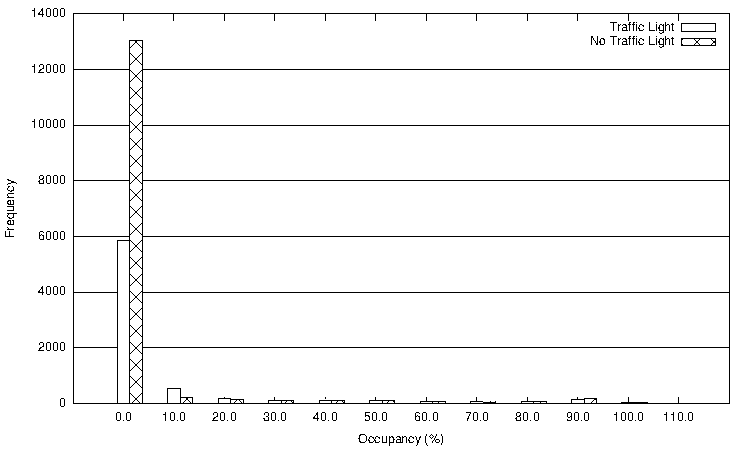
\includegraphics[width=0.75\textwidth]{figs/ss_hist_occup.pdf}
	\caption{Histograma da Taxa de Ocupação com e sem sinais}
	\label{fig:hist-occup}
\end{figure}

\begin{Verbatim}[numbers=left]
String setupName = "segmentspeed2.SUMOTrafficSpeedSetup"
String inDir = "results/segmentspeed2/rateresults"
String outDir = "results/segmentspeed2/ss_occupancy"
rates = [100]
String metricName = "hist_occup_tl"
...
def meanerror = rates.collect{[it,
	run(it, {vals-> vals.edgetl.equals("1")}, binfOccup, {1}, outfStats )] 
}
\end{Verbatim}

Na linha 8, a chamada à função \tm{run} especifica no 2º argumento o filtro para segmentos com semáforo. O 3º argumento é a função de classificação por taxa de ocupação. Segue-se a função de sumarização que neste caso não é relevante - é uma função que devolve sempre o valor 1 - estamos interessado apenas na frequência de ocorrência.  

Para obter os dados para segmentos sem sinais, altera-se apenas o nome da métrica (define o nome dos ficheiros de output) e a função de filtragem como se segue:

\begin{Verbatim}[numbers=left]
...
String metricName = "hist_occup_notl"
...
def meanerror = rates.collect{[it,
	run(it, {vals-> vals.edgetl.equals("0")}, binfOccup, {1}, outfStats )] 
}
\end{Verbatim}

A frequência de cada classe será a 4ª coluna dos ficheiro de output. O seguinte script gnuplot constroi o gráfico da figura \ref{fig:hist-occup}:

\begin{Verbatim}[numbers=left]
set term pdf monochrome
set output "ss_hist_occup.pdf"
set style histogram clustered
set style fill pattern
set grid ytics
set xlabel "Occupancy (%)"
set ylabel "Frequency"
plot "ss_hist_occup_tl_100.gpd" u 4:xtic(1) w histogram t "Traffic Light",\
	"ss_hist_occup_notl_100.gpd" u 4 w histogram t "No Traffic Light"
\end{Verbatim}



%%%%%%%%%%%%%%%%%%%%%%%%%%%%%%%%%%%%%%%%%%%%%%%%%%%%%%%%%%%%%%%%%%%%
% Backup
%%%%%%%%%%%%%%%%%%%%%%%%%%%%%%%%%%%%%%%%%%%%%%%%%%%%%%%%%%%%%%%%%%%%
\begin{comment}
\section{Preparação de uma Simulação}\label{sec:preparacao}

\subsection{Simulador}

Um simulador é uma extensão da classe Groovy \tm{sensing.persistence.simsim.PipelineSimulation}. Criar um novo tipo de aplicação -  \eg SpeedSense baseado em OSM, SpeedSense SUMO, NoiseMap, etc.. - passa por criar um simulador que cria as estruturas necessárias para a aplicação. Como exemplo, descreve-se a seguir a classe abstracta \tm{SpeedSenseSim}, e a especialização \tm{SUMOSpeedSenseSim} para a aplicação SpeedSense baseado no SUMO.




\subsubsection{SpeedSenseSim}

A classe \tm{SpeedSenseSim} 


\subsubsection{SUMOSpeedSenseSim}

No construtor é definida estratégia de distribuição:

\begin{Verbatim}
QUERY_IMPL_POLICY = ServicesConfig.QueryImplPolicy.CENTRALIZED;
\end{Verbatim}

No método \tm{init} são cr



\subsection{Nós Moveis}

Um novo tipo de nó móvel é definido por extensão da classe Java \tm{sensing.persistence.simsim.MobileNode}. A extensão de \tm{MobileNode} define o comportamento do nó e utiliza o método \tm{sensorInput} para comunicação de leituras. Como exemplo de nó móvel, ver  \tm{sensing.persistence.simsim.sumo.SUMOMNodeSegmentSpeed2}. \

A comunicação de uma tuplo segue a seguinte lógica:

\begin{Verbatim}
GroovyObject m = simJ.newTuple("speedsense.MappedSpeed"); 
m.setProperty("segmentId", sampledEdge.id); 
...
sensorInput(m);
\end{Verbatim}

O metodo \tm{sensorInput} será responsável por acrescentar o timestamp e identificador do nó móvel.



\subsection{Tabelas Virtuais}


\subsection{Setup}

\end{comment}


%%%%%%%%%%%%%%%%%%%%%%%%%%%%%%%%%%%%%%%%%%%%%%%%%%%%%%%%%%%%%%%%%%%%%%
%% Finally we specify the format required for our references and the
%% name of the bibtex file where our references should be taken from.
%%%%%%%%%%%%%%%%%%%%%%%%%%%%%%%%%%%%%%%%%%%%%%%%%%%%%%%%%%%%%%%%%%%%%%

\bibliographystyle{plainnat}
\bibliography{example}

\end{document}

%%%%%%%%%%%%%%%%%%%%%%%%%%%%%%%%%%%%%%%%%%%%%%%%%%%%%%%%%%%%%%%%%%%%%%
%% The end.
%%%%%%%%%%%%%%%%%%%%%%%%%%%%%%%%%%%%%%%%%%%%%%%%%%%%%%%%%%%%%%%%%%%%%%